\documentclass[russian,utf8,a1paper,portrait,nostitching,simple]{eskdgraph}
\usepackage[T2A]{fontenc}
\usepackage{pscyr}
\usepackage{tikz}
\usepackage{color}

\newcommand{\No}{\textnumero}

\ESKDunitName{Схема алгоритма инициализации программного модуля}
\ESKDsignature{ГУИР.000000.005 ПД}
\ESKDletter{}{Т}{}
\ESKDauthor{Анашкевич}
\ESKDchecker{Барановский}
\ESKDcolumnXIfIII{Павловская}
\ESKDnormContr{Протченко}
\ESKDapprovedBy{Навроцкий}
\ESKDgroup{ИТАС, гр. 120602}

\renewcommand{\ESKDcolumnXfIVname}{Реценз.}
\ESKDcolumnXIfIV{}

\begin{document}

\ESKDthisStyle{formI}
\begin{ESKDdrawing}
  \centering
  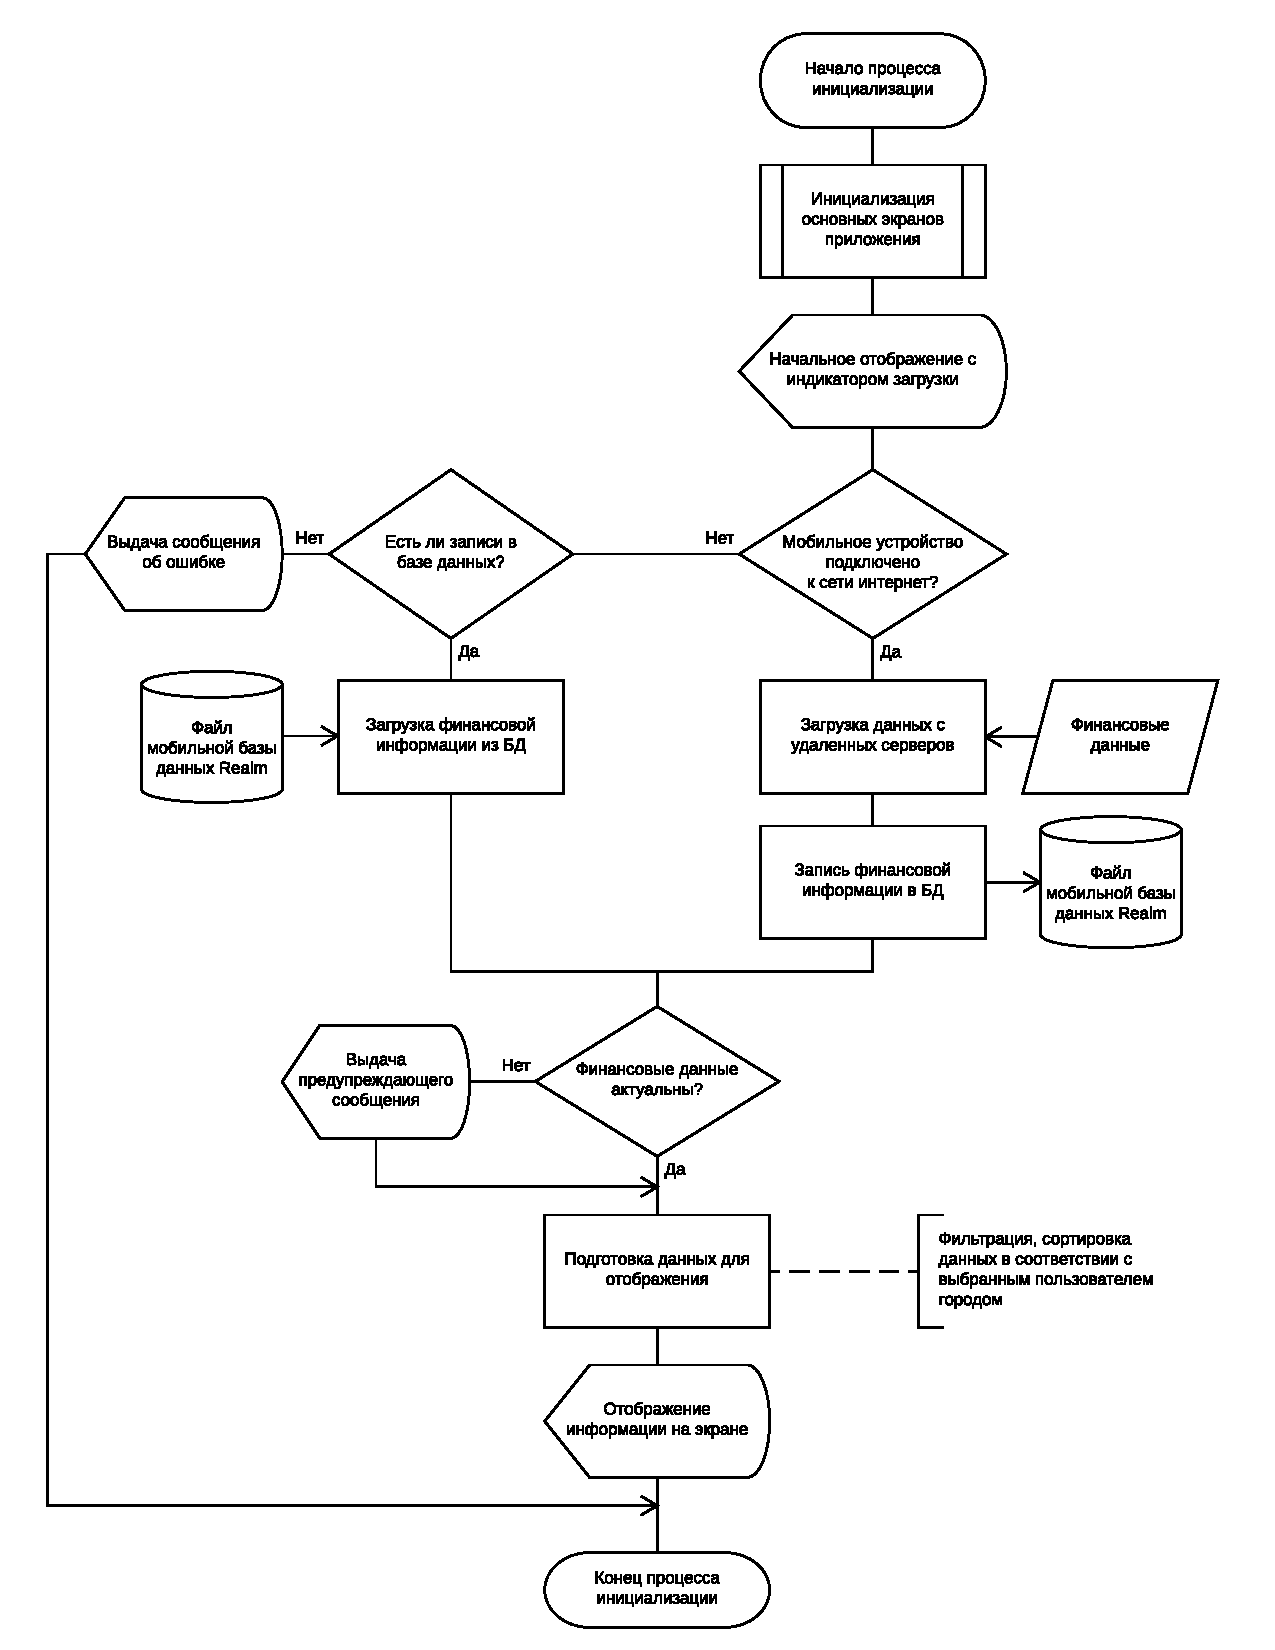
\includegraphics[height=70cm]{fig/module_initialization.pdf}
\end{ESKDdrawing}

\end{document}
